% As the third use-case, we have implemented the
DVMS (Distributed Virtual Machine Scheduler)~\cite{quesnel:cpe2012} enables the
cooperative and fully-distributed placement of
VMs. A DVMS agent is deployed on each node in order to manage the VMs on
the node and collaborate with (the agents of) neighboring nodes.
Agents are defined on top of an overlay communication network that
defines the node-neighbor relation.
% and can be structured (using, \eg
% Chord~\cite{stoica:2001:sigcomm01}) or unstructured.  For this
% study,
We have implemented a simple % but effective
unstructured overlay that enables the agents to collaborate
% without side effects: when necessary, \eg in case of node failures,
% the overlay
by providing a link to a neighbor %of a node
on the latter's request.
% \MS[AL, JP]{A bit short. What about an architecture figure (as for
%  Snooze?)}




% \paragraph{Iterative Scheduling Procedure.}
% \label{sec:ISP}
% \AL[MS,JP]{if we succeed to have only one or two subsections in
%   Snooze, we should do the same here.}

Fig. \ref{fig:dvms_pte} depicts the DVMS algorithm.
When a node N\(_{\textit{i}}\) detects that it cannot provide enough
resources for its hosted VMs, %(\ie VMs hosted on the server require more
%resources than available),
an \emph{Iterative Scheduling Procedure
  (ISP}) is started:
%
%When a node N\(_{\textit{i}}\)
%detects that it cannot provide enough resources for its hosted VMs,
it initiates a partition, reserving itself to solve the problem, see
Fig.~\ref{fig:dvms_pte_1}.  Then, its closest
neighbor % , as defined by the network overlay,
is considered.
%
%
%
If this neighbor, N\(_{\textit{i+1}}\),
is already part of another partition, the next neighbor is considered.
%\AL[MS]{Not clear enough, its next neighbor ?}
Otherwise, N\(_{\textit{i+1}}\)
joins the partition (see Fig.~\ref{fig:dvms_pte_2}) and becomes the
partition leader.
% % If the partition is not valid anymore (\eg because the workload of the
% % partition's VM has decreased), N\(_{\textit{i+1}}\)
% % cancels the reservations, destroys the partition and thus frees its
% % nodes for another problem solving procedure.
% % %
% % On the contrary, if the procedure is still valid, N\(_{\textit{i+1}}\)
% % notifies members of the partition that it has become the new
% % leader.
%

The other nodes involved in the partition then send it information about their
capacities and current load. The leader, in turn, starts a scheduling
computation looking for a reconfiguration within the current
partition. If no solution is found, the same algorithm is applied to
the next node N\(_{\textit{i+2}}\).
%
% % In the extreme case a partition may grow until all resources in a
% % cluster contribute to the resolution of its resource scheduling
% % problem.
This approach constructs small partitions in a highly parallel manner
(Fig.~\ref{fig:dvms_pte_3}), thus accelerating the scheduling process
and reactivity.

\begin{figure}[hbp]
\vspace*{-.4cm}
\subfigure[]{
\hspace*{-.6cm}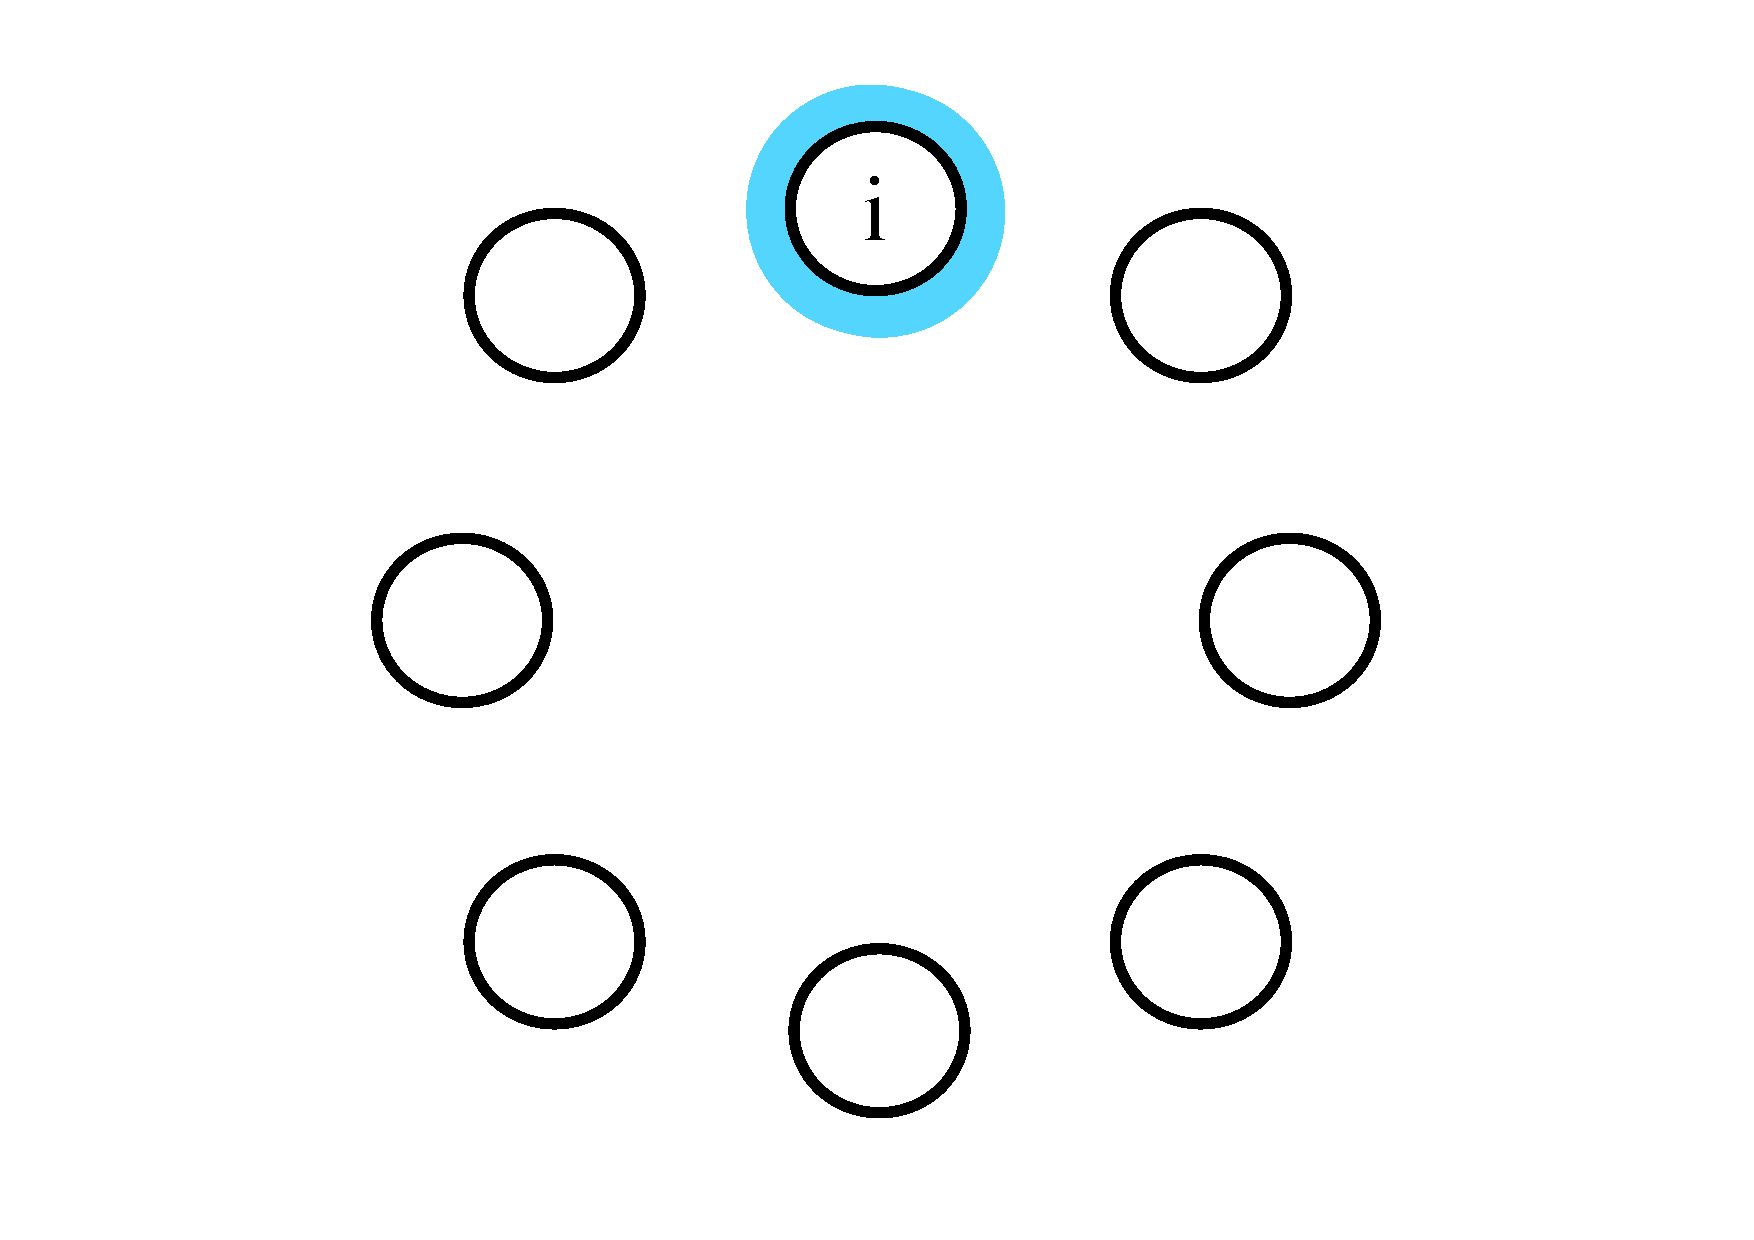
\includegraphics[width=3.3cm]{./figures/fig-24.pdf}
\label{fig:dvms_pte_1}}
%
\subfigure[]{
\hspace*{-.8cm}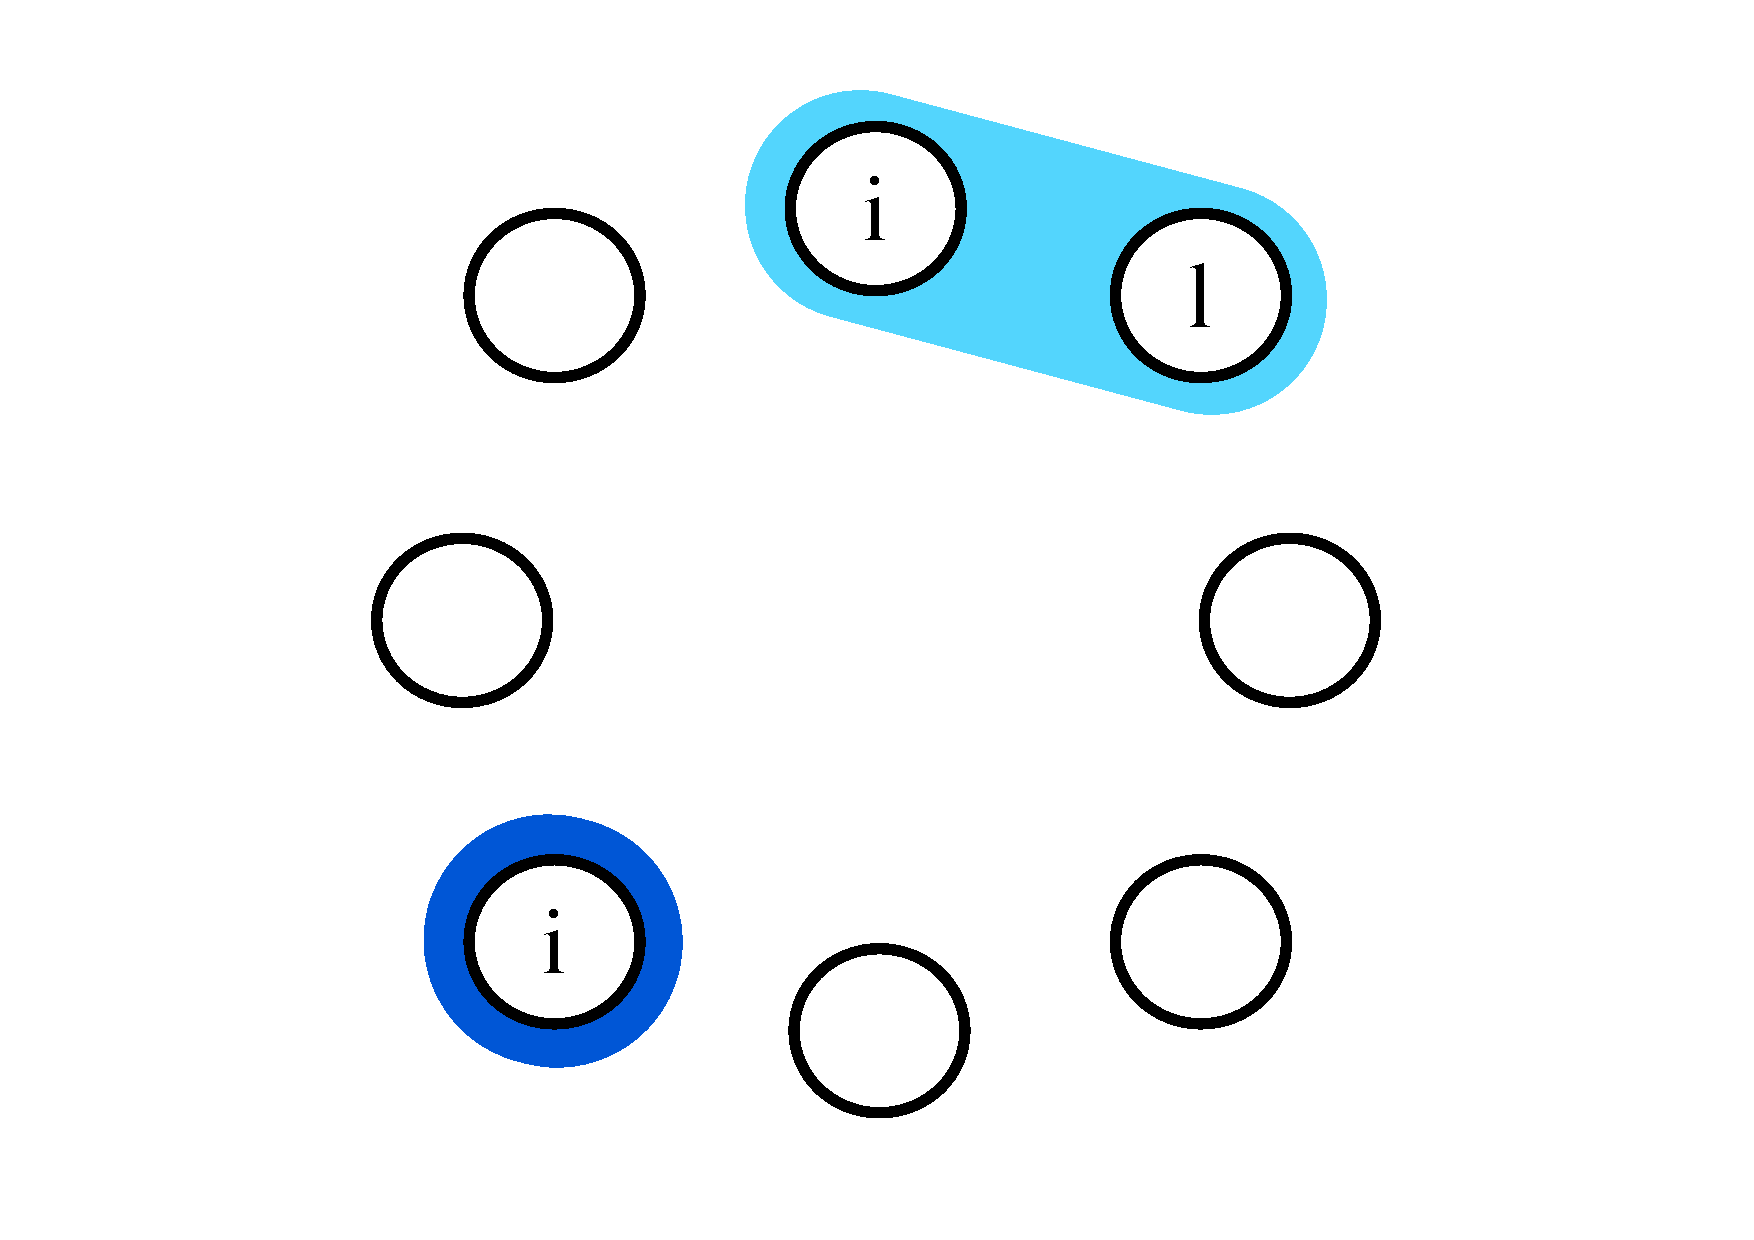
\includegraphics[width=3.3cm]{./figures/fig-25.pdf}
\label{fig:dvms_pte_2}}
%
\subfigure[]{
\hspace*{-.8cm}
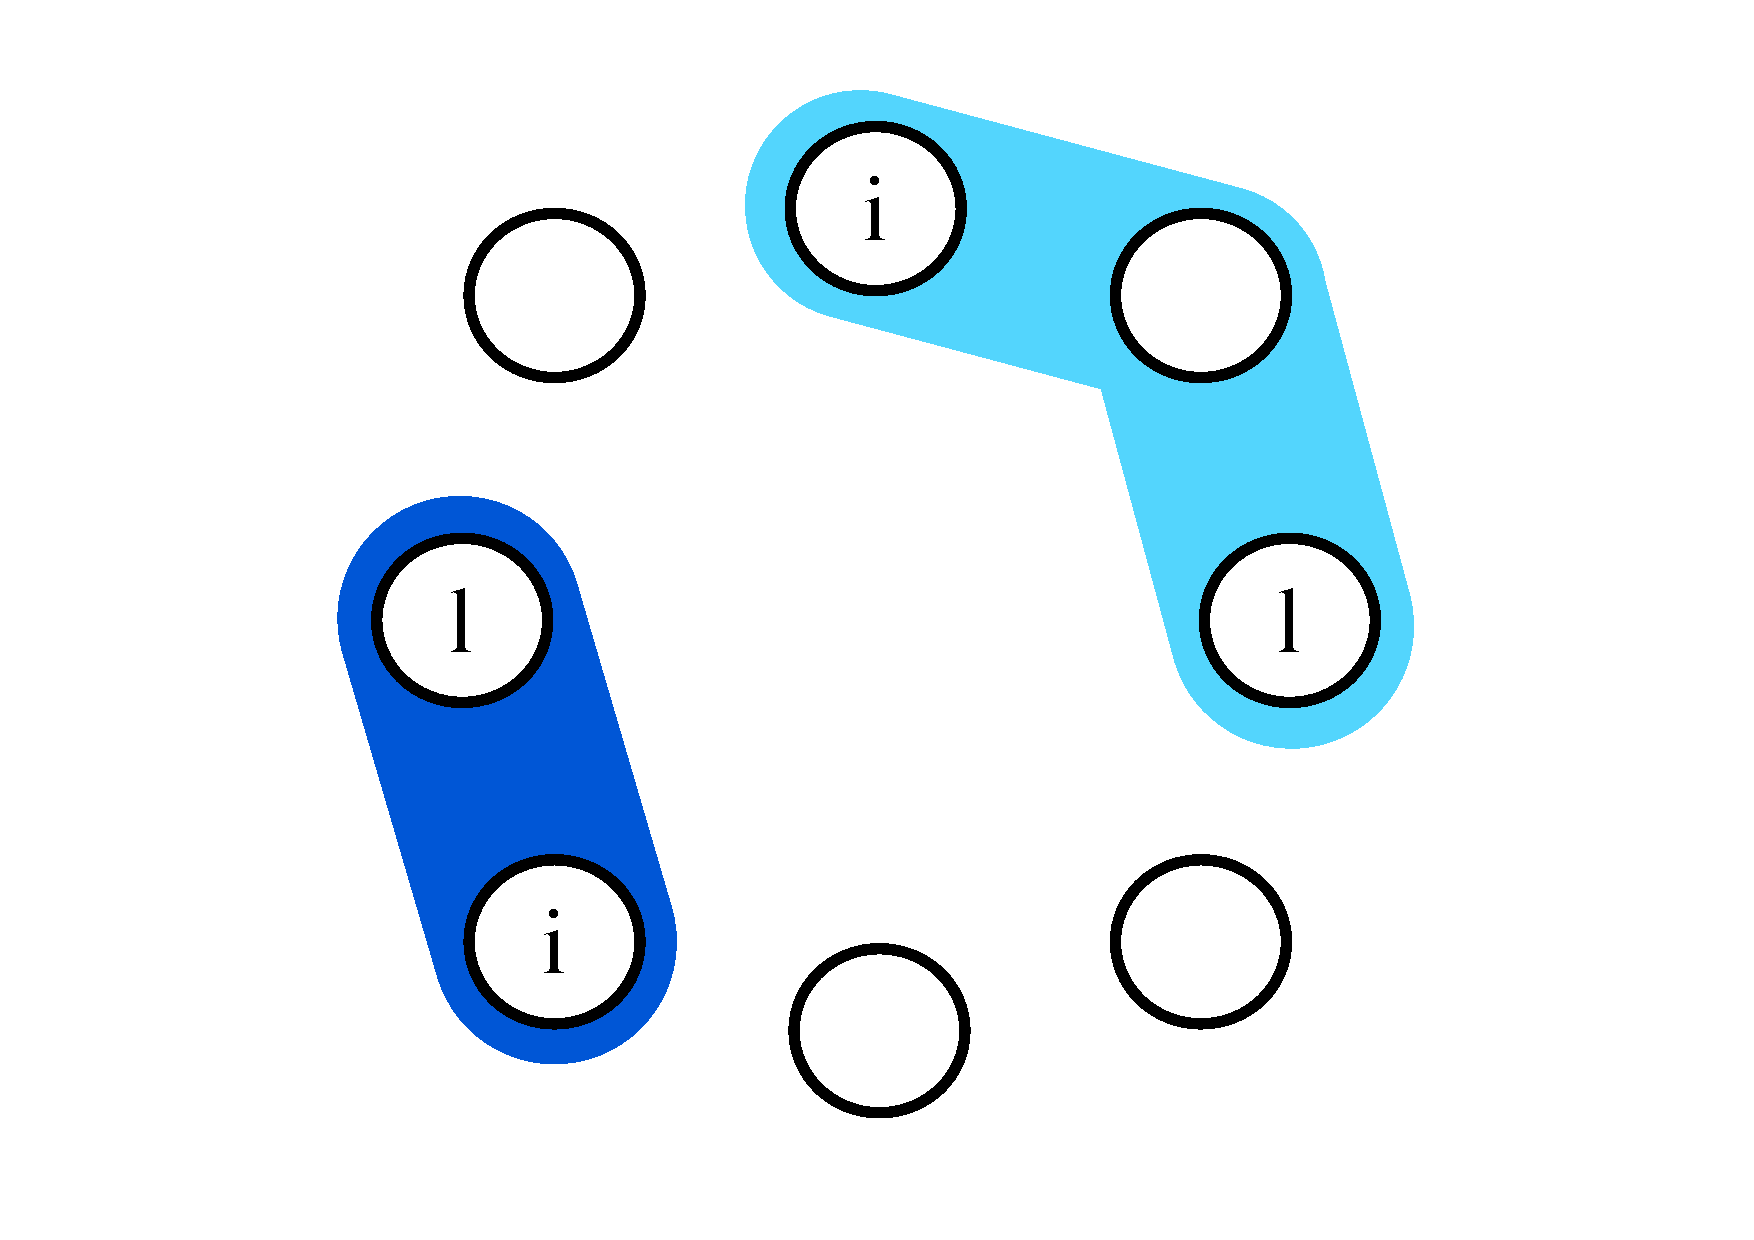
\includegraphics[width=3.3cm]{./figures/fig-26.pdf}
\label{fig:dvms_pte_3}}
%
\subfigure[Legend]{
\hspace*{-.6cm}
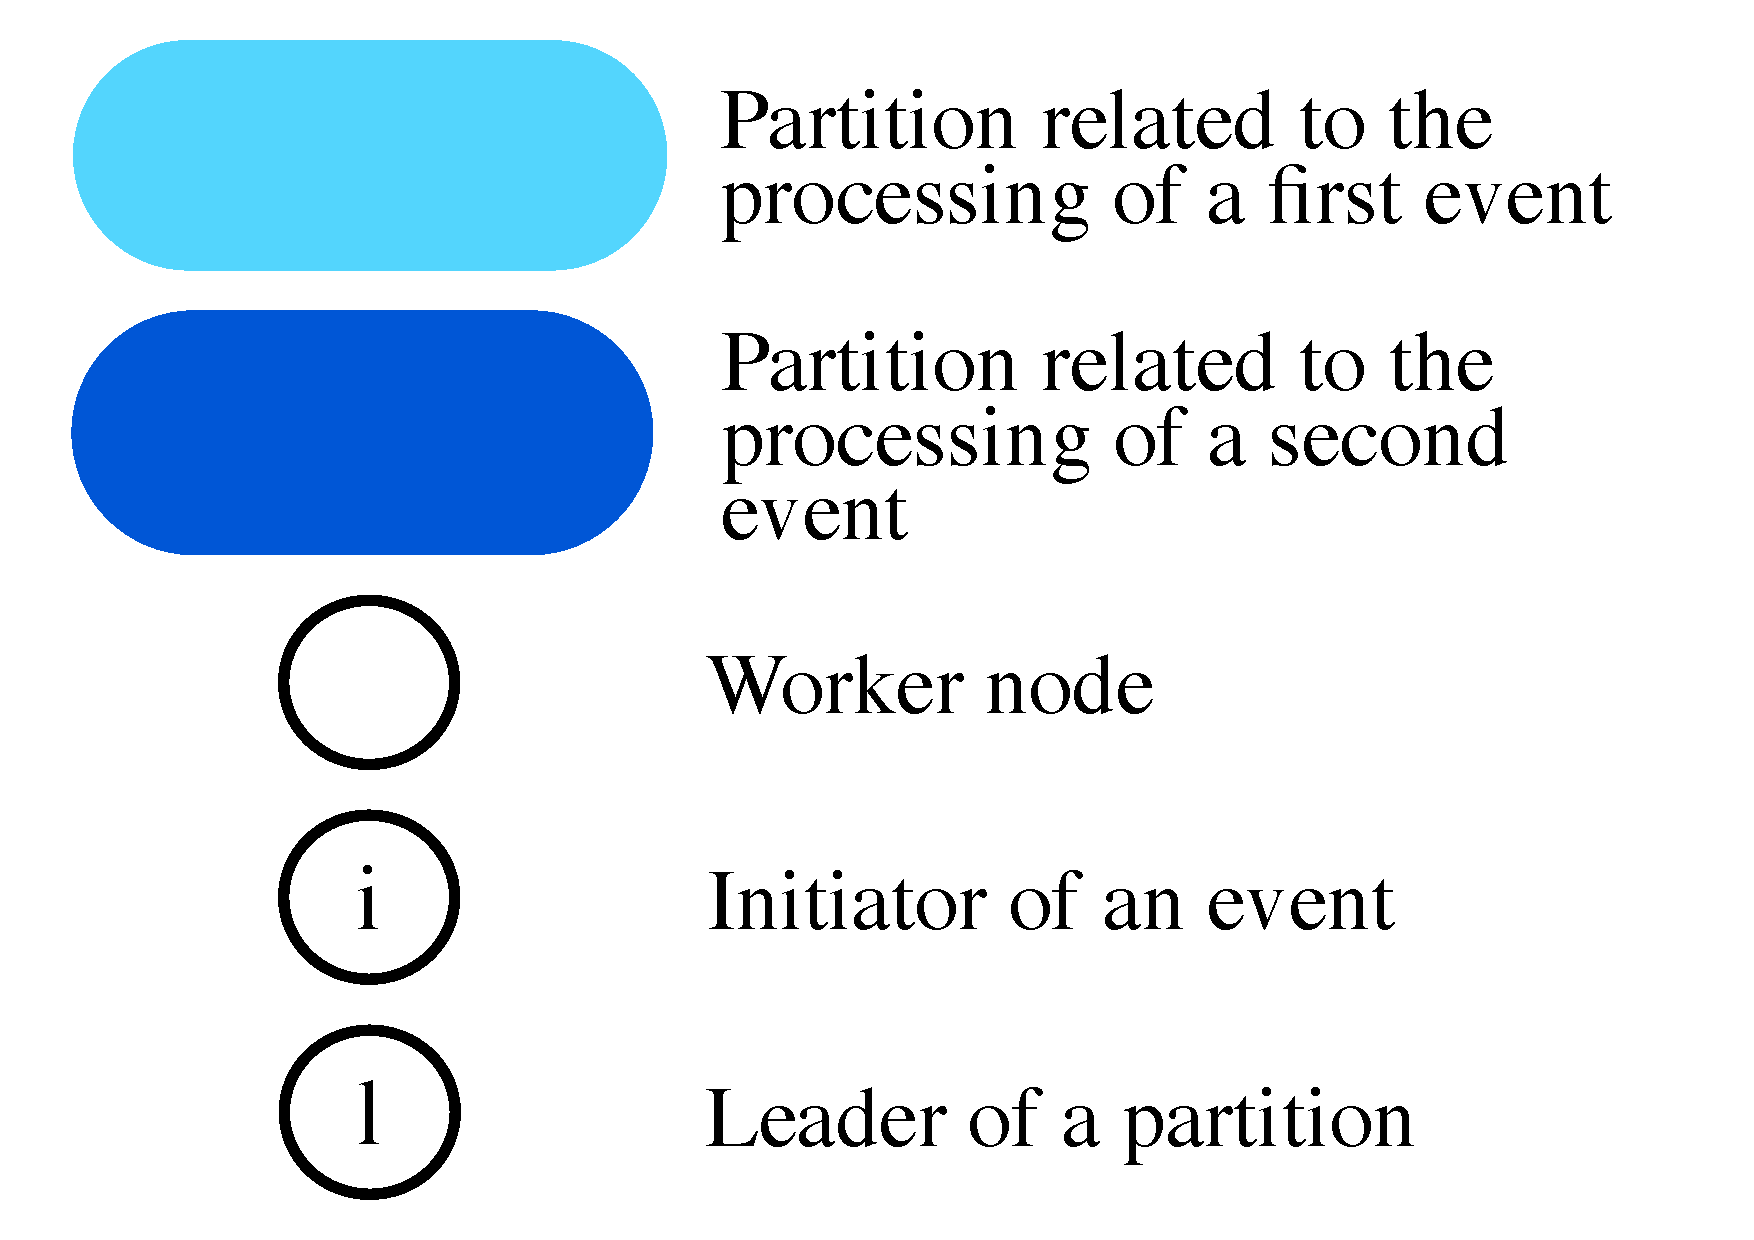
\includegraphics[width=3.3cm]{./figures/fig-27.pdf}
\label{fig:dvms_pte_4}}
%
\vspace*{-.4cm}
\caption{Processing two events simultaneously\label{fig:dvms_pte}}
\vspace*{-1cm}
\end{figure}

Most of the DVMS code has been coded in SCALA leveraging the Java
primitives of \sg for the communications between the different DVMS
agents that have been implemented, in turn, using the abstractions of \vmps.


% \subsubsection{Fault-tolerance}

% The main advantage of using overlay networks is that they have
% built-in fault tolerance mechanisms. DVMS therefore works on top of an
% overlay network such as Chord: when a node needs to rebalance its VMs
% workload, it uses the overlay network to find collaborators. For this
% study we implemented a simple overlay network as a flat list of
% agents: a typical request for collaborators includes the list of
% agents that are already collaborating with the requesting agent. A
% link to a new collaborator is then provided to the requesting
% agent. Communication is performed by message exchanges containing
% immutable data: our implementation harnesses the principles of the
% actor model in order to ease the handling of concurrency and
% distributed issues.

% Even if the implementation of the overlay network is simple, it
% fulfills its purpose, and in the case where one would want to use a
% different overlay network such as a ring topology, it only has to
% reuse the API provided by this simple implementation, and adapts its
% functionning to the targeted overlay network.
% \AL[JP]{here we do not describe DVMS in general but we should
% emphasize what has been exactly implemented and how} \JP[AL]{I added
% the preceding paragraph that gives more details about the overlay
% network used.}
%
% This functionning allows firstly a loosely coupling between DVMS and
% the overlay network used, and, secondly, to delegate most of the
% fault tolerance mechanisms to the overlay network. Although
% leveraging an overlay network to address node crashes is helpfull,
% it is not enough to make the problem solving procedure
% fault-tolerant.

% Harnessing the fault tolerance mechanisms of the underlying overlay
% network is, however, not sufficient. If the leader of a partition
% crashes, a new leader must take over in order for the resource problem
% to be solved and the nodes of a partition to be finally freed.  To
% avoid these issues, DVMS now relies on timeout mechanisms.  Each node
% of a partition periodically checks whether the state of its partition
% changed recently (\eg, if a new node joined the partition) and can
% thus identify if the partition's leader is not active anymore.  In
% this case, each node leaves the partition and can be integrated in
% other partitions.

%%% Local Variables:
%%% mode: latex
%%% TeX-master: "main"
%%% End:
